\documentclass[twoside]{article}
\usepackage{amssymb}
\usepackage{amsthm}
\usepackage{amsmath}
\usepackage{amsfonts}
\usepackage[utf8]{inputenc}
\usepackage[spanish]{babel}
\usepackage{tikz}
\usepackage{centernot}
\usepackage{hyperref}
\usepackage{fancyhdr}
\usepackage{lipsum}
\usepackage{subcaption}
\usepackage{pgfplots} 
\hypersetup{
    colorlinks,
    citecolor=black,
    filecolor=black,
    linkcolor=black,
    urlcolor=black
}
\usepackage{xurl}
\usepackage[top=1in, bottom=1.5in, left=1in, right=1in]{geometry}
\pagestyle{fancy}
\fancyhead{}
\fancyhead[L]{\leftmark}
\fancyfoot{}
\fancyfoot[C]{\thepage}
\newcommand{\enquote}[1]{``#1''}
\usepackage{float}
\usepackage[parfill]{parskip}
\newcommand{\image}[2]{
\begin{figure}[H]
    \includegraphics[width=#1 cm]{../images/#2.png}
    \centering
\end{figure}
}

\title{Práctica 3 SWAP}
\author{XuSheng Zheng}
\date{}

\begin{document}

\maketitle
\tableofcontents
\newpage

\section{Creación de la tercera máquina}
Para esta práctica, necesitamos crear una tercera máquina virtual que nos servirá de balanceador. Para ello, especificamos los siguientes datos siguiendo los mismos pasos que en la práctica 1:
\image{8}{1}
Una vez instalada la máquina, necesitamos configurar la conexión a red. Lo hacemos de la misma manera que en la práctica 1:
\image{8}{2}
Y comprobamos con \textbf{ifconfig}:
\image{8}{3}


\section{Nginx}
Instalamos \textbf{nginx} en m3 mediante \textbf{apt-get} con los comandos del guion y comprobamos que está activado:
\image{8}{4}
Ahora procedemos a la configuración: en primer lugar deshabilitamos la funcionalidad de servidor web editando en \textit{/etc/nginx/nginx.conf} comentando la línea \textit{include /etc/nginx/sites-enabled/*;} :
\image{8}{5}
Creamos el archivo de configuración \textit{/etc/nginx/conf.d/default.conf} con los siguientes datos:
\image{8}{6}
Una vez guardado, reiniciamos el servicio \textbf{nginx}. Para comprobar el funcionamiento del balanceador, se ha modificado el archivo \textit{/var/www/html/swap.html} para que se pueda distinguir las máquinas:
\begin{figure}[H]
    \centering
    \begin{subfigure}{.5\textwidth}
        \centering
        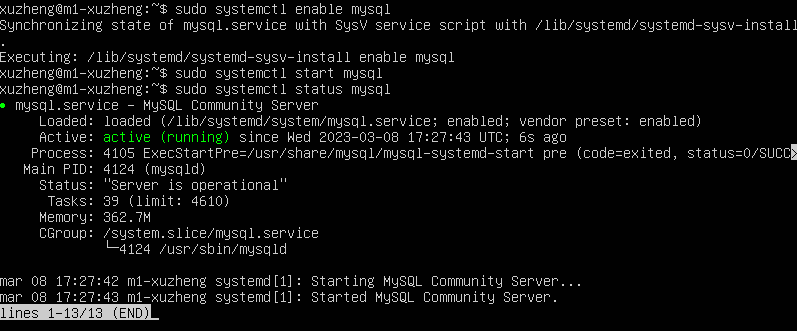
\includegraphics[width=7cm]{../images/10.png}
    \end{subfigure}%
    \begin{subfigure}{.5\textwidth}
        \centering
        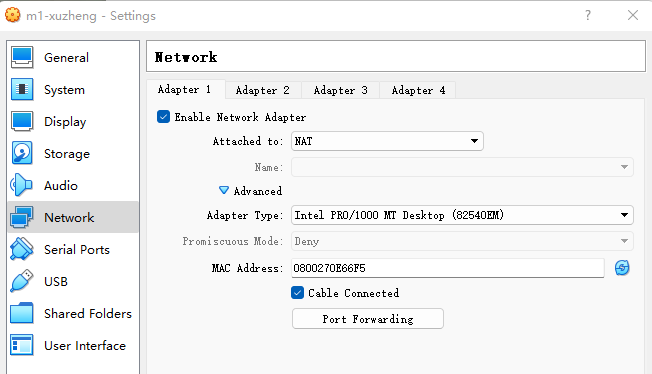
\includegraphics[width=7cm]{../images/11.png}
    \end{subfigure}
\end{figure}
Ahora podemos comprobar el funcionamiento de \textbf{nginx} usando \textbf{cURL} desde el anfitrión:
\image{8}{7}
En este caso hemos tratado las dos máquinas por iguales. Podemos dar más peso a la primera máquina mediante el modificador \textbf{weight}:
\image{8}{8}
Ahora de cada 3 peticiones, 2 serán atendidas por m1 y 1 por m2:
\image{8}{9}

\subsection{Opciones avanzadas}
Para evitar el conflicto de estados y sesiones entre los servidores, \textbf{nginx} permite dirigir las peticiones provenientes de un determinado IP al mismo servidor final mediante la opción \textbf{ip\_hash}. 

La directiva \textbf{keepalive} determina el número máximo de conexiones a servidores finales que se mantiene en caché y \textbf{keepalive\_requests} determina el número máximo de peticiones que pueden servir a través de estas conexiones, una vez que el número de peticiones exceda el máximo, la conexión se cerrará.
\image{8}{12}
Comprobamos el funcionamiento a través del anfitrión:
\image{8}{13}
Podemos que en este caso sólo sirve m2 pues estamos enviando a través del mismo IP.

Para gestionar caídas de los servidores podemos usar los comandos \textbf{max\_fails} para especificar el número máximo de intentos de comunicación fallidos antes de considerar al servidor no operativo y \textbf{fail\_timeout} para especificar el periodo de tiempo con el que se considera esos intentos. En el siguiente ejemplo consideramos que el servidor no será operativo si existen 3 intentos fallidos en un periodo de 30 segundos:
\image{8}{14}


\section{Haproxy}
Para este apartado, paramos y desactivamos \textbf{nginx} para evitar conflictos e instalamos \textbf{haproxy} mediante \textbf{apt-get}.
\image{8}{15}
Comprobamos que está activo:
\image{8}{16}
Pasamos ahora a configurar \textbf{haproxy}: añadimos al archivo \textit{/etc/haproxy/haproxy.cfg} las siguientes líneas para tener una configuración round-robin básica:
\image{8}{17}
Reiniciamos el servicio y comprobamos desde el anfitrión:
\image{6}{18}
Para dar más peso a determinados servidores, podemos usar la opción \textbf{weight} con números entre 0 y 256 en las líneas de \textbf{server}. Para tener la analogía con el apartado de \textbf{nginx}, asignamos a m1 el doble de carga que m2:
\image{8}{19}
Y comprobamos:
\image{6}{20}
Vemos que efectivamente m1 atiende 2 de las 3 peticiones.
\subsection{Opciones avanzadas}
Al igual que \textbf{nginx}, \textbf{haproxy} también permite el balanceo por IP mediante la opción \textbf{hash-type consistent}.

Además, \textbf{haproxy} permite 3 tipos de comprobaciones sobre el estado de los servidores:
\begin{itemize}
    \item Activo: por defecto en este caso \textbf{haproxy} intentará establecer una conexión TCP con el servidor final cada 2 segundos. Tras 3 conexiones fallidas se considerará que el servidor está caído y no se le enviará peticiones hasta que consiga 2 conexiones exitosas.
    \item Pasivo: similar a la opción \textbf{keepalive\_requests} de \textbf{nginx}, establece un límite de errores consecutivos que puede haber antes de dar por caído al servidor.
    \item Agente: mediante un agente externo del servidor final, \textbf{haproxy} puede controlar el estado con el que se encuentra el servidor.
\end{itemize}
En el siguiente ejemplo establecemos un máximo de 10 errores:
\image{8}{21}
Con \textbf{observe layer7} indicamos que se consideren todas las respuestas HTTP del servidor y con \textbf{on-error mark-down} indicamos que el servidor esta caído cuando se alcance los 10 errores.
Para comprobar el funcionamiento del balanceo por IP, mandamos peticiones desde el anfitrión:
\image{6}{22}
Podemos apreciar que todas las peticiones son atendidas por m1 pues provienen del mismo IP.

\section{Módulo de estadísticas}
Para habilitar el módulo de estadísticas de Haproxy, añadimos las siguientes líneas al archivo \textit{/etc/haproxy\\/haproxy.cfg}:
\image{8}{23}
Reiniciamos el servicio y ahora podemos acceder a través de la url \textit{http://192.168.56.72:9999/stats} con el usuario y la contraseña que hemos configurado:
\image{10}{24}
Para poder testear el módulo de estadísticas, deshabilitamos de momento el balanceo por IP:
\image{8}{25}
Tras reiniciar el servicio lanzamos varias peticiones al balanceador y observamos los datos recogidos por el módulo son correctos:
\begin{figure}[H]
    \centering
    \begin{subfigure}{.3\textwidth}
        \centering
        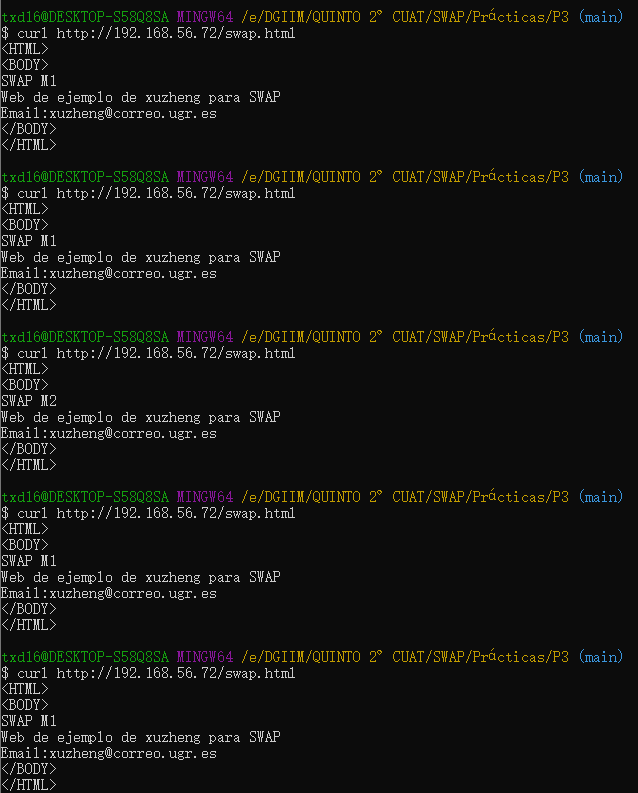
\includegraphics[width=4.5cm]{../images/26.png}
    \end{subfigure}%
    \begin{subfigure}{.7\textwidth}
        \centering
        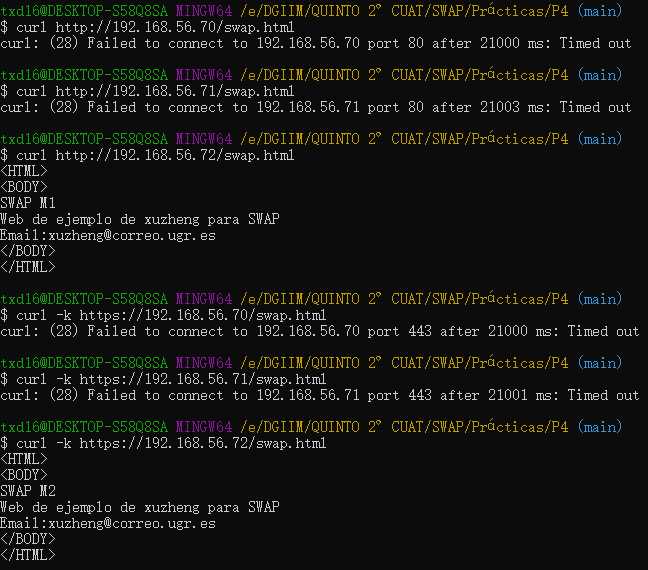
\includegraphics[width=10.5cm]{../images/27.png}
    \end{subfigure}
\end{figure}
En particular se verifica que m1 haya servido 4 de las 5 peticiones.
\subsection{Opciones avanzadas}
Para que la página de estadísticas se actualice automáticamente podemos usar \textbf{stats refresh} con el periodo de tiempo con el que queremos que se actualice. Para limitar el número de conexiones a la página podemos usar \textbf{stats maxconn} y se puede establecer un timeout mediante \textbf{stats timeout}. 

En el siguiente ejemplo establecemos un refresco de página por cada 10 segundos, un timeout de 30 segundos y un número máximo de 5 conexiones:
\image{8}{28}

\section{Go-Between}
Para evitar conflictos, deshabilitamos los balanceadores anteriores e instalamos \textbf{go-between} mediante \textbf{sudo snap install gobetween --edge}. Una vez instalado comprobamos el estado del servicio:
\image{8}{29}
Para configurar el algoritmo roundrobin editamos el archivo \textit{/var/snap/gobetween/common/gobetween.toml} como sigue:
\image{6}{30}
Además, para evitar errores, se ha desactivado el servidor de API REST y el servidor de ejemplo para UDP:
\begin{figure}[H]
    \centering
    \begin{subfigure}{.5\textwidth}
        \centering
        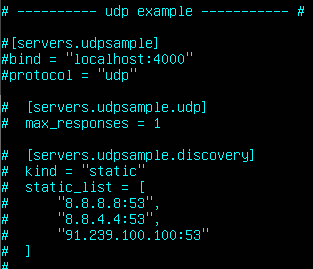
\includegraphics[width=7cm]{../images/31.png}
    \end{subfigure}%
    \begin{subfigure}{.5\textwidth}
        \centering
        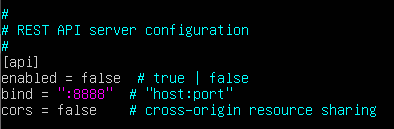
\includegraphics[width=7cm]{../images/32.png}
    \end{subfigure}
\end{figure}
Para efectuar la configuración ejecutamos lo siguiente:
\image{8}{33}
Y comprobamos desde el anfitrión:
\image{8}{34}
\subsection{Opciones avanzadas}
\textbf{go-between} también permite el balanceo por IP mediante la opción \textbf{balance=\enquote{iphash}} así como ponderación mediante \textbf{balance=\enquote{weight}}. Para seguir el mismo esquema de los anteriores balanceadores damos el doble de carga para m1:
\image{6}{35}
Lanzamos el servicio y comprobamos desde el anfitrión:
\image{8}{36}
A diferencia de los anteriores balanceadores, que determinan el peso de cada máquina en roundrobin, en este caso la ponderación determina la probabilidad de ser elegida para servir una petición. Lo que implica que no tenemos asegurado que de las 3 peticiones, 2 vayan a ser servidas por m1.
Para controlar el estado de los servidores finales, \textbf{go-between} hace uso del apartado \textbf{healthcheck}. Veamos con el siguiente ejemplo:
\image{6}{37}
Con esta configuración estamos indicando que se realice un chequeo sobre el estado de los servidores por cada 5 segundos mediante conexiones por \textbf{ping}. Si una conexión no se establece en 500 ms se considera una pérdida. Tras 3 pérdidas, se considerará que el servidor esta caído. Mientras que 2 conexiones exitosas a un servidor caído se considerará que se ha recuperado.  

Para evitar conflicto con el siguiente balanceador, deshabilitamos \textbf{gobetween} con el comando \textbf{sudo snap disable gobetween}.

\section{Pound}
Actualmente no se puede instalar \textbf{pound} mediante \textbf{apt-get}, pero se ha encontrado un repositorio que almacena archivos para la instalación \textbf{pound}. Dado que la versión de nuestro Ubuntu es la 18, la versión de \textbf{pound} que nos funciona es la 2.6.

Por tanto, descargamos el archivo \textit{pound\_2.6-2\_amd64.deb} de \url{http://old.kali.org/kali/pool/main/p/pound/} con el comando \textbf{curl -O http://old.kali.org/kali/pool/main/p/pound/pound\_2.6-2\_amd64.deb} e instalamos el paquete con \textbf{sudo dpkg -i pound\_2.6-2\_amd64.deb}. Una vez instalado podemos comprobar su estado:
\image{8}{38}
Para configurar, editamos el archivo \textit{/etc/pound/pound.cfg}:
\image{8}{39}
Al reiniciar el servicio nos pide que añadamos \textbf{startup=1} al documento \textit{/etc/default/pound}:
\image{8}{40}
Lo añadimos y reiniciamos el servicio.
\image{8}{41}
\image{8}{42}
Comprobamos que funciona correctamente desde el anfitrión:
\image{8}{43}
También podemos otorgar más prioridad para una máquina que otra:
\image{8}{44}
\subsection{Opciones avanzadas}
Para establecer el balanceo por IP podemos utilizar el bloque \textbf{session}, éste nos permite configurar el tiempo máximo en el que se mantiene una sesión, en nuestro caso se ha decidido un margen de 20 minutos:
\image{8}{45}
Comprobamos desde el anfitrión:
\image{8}{46}
Para controlar el estado de los servidores, se puede configurar las directivas globales \textbf{TimeOut} y \textbf{ConnTO} que establecen el tiempo que espera \textbf{Pound} para una respuesta del servidor y una conexión al servidor respectivamente. Estas directivas se pueden sobreescribir en cada servidor. Además, \textbf{Alive} determina cada cuánto tiempo \textbf{Pound} chequea el estado de los servidores. En nuestro caso asignamos los siguientes valores:
\image{6}{47}

\section{Someter a carga la granja web con AB}
A partir de esta sección, se ha eliminado la configuración respecto al balanceo por IP de todos los balanceadores.

En primer lugar instalamos \textbf{Apache Benchmark} en el anfitrión. Dado que en este caso el anfitrión tiene el sistema operativo Windows, se ha seguido los pasos del videotutorial \url{https://www.youtube.com/watch?v=hUZso9TpEes}.

Una vez instalado probamos solicitar 10000 veces la página \textit{swap.html} en peticiones concurrentes de 10 en 10:
\image{8}{48}
Podemos ver que en este caso el tiempo medio por petición es de 50 ms.
\subsection{Otras opciones}
Aparte de las opciones \textbf{-n} y \textbf{-c} visto anteriormente, \textbf{ab} tiene otras opciones interesantes:
\begin{itemize}
    \item \textbf{-e csv-file}: escribe en un csv el tiempo que se tardó para procesar cada porcentaje de las peticiones totales.
    \item \textbf{-q}: elimina los mensajes de progreso.
    \item \textbf{-p, -u file}: permite añadir fichero con datos para peticiones POST y PUT respectivamente. Es necesario usar también la opción \textbf{-T}. 
    \item \textbf{-t timelimit}: determina el número máximo de segundos para el benchmark.
\end{itemize}
Como ejemplo utilizamos el siguiente comando:
\image{8}{49}
Podemos ver que en este caso ya no nos muestra el mensaje sobre el número de peticiones completas y si abrimos \textit{ejemplo.csv} tenemos lo siguiente (se muestra sólo una parte del csv):
\image{6}{50}

\section{Análisis comparativo de los balanceadores}
A continuación presentamos los resultados de los balanceadores sometiéndolos a una carga de 10000 peticiones concurrentes de 10 en 10. Para cada balanceador se testea tanto con roundrobin como con ponderación con m1 el doble de carga que m2.
 \begin{center}
    \begin{tabular}{|c|c|c|c|c|}
        \hline
        Balanceador & Algoritmo & Tiempo total (s) & Peticiones/s & Longest request (ms) \\
        \hline
        Nginx & RoundRobin & 57.038 & 175.32 & 563 \\
        \hline
        Nginx & Ponderación & 55.867 & 179.00 & 542 \\
        \hline
        Haproxy & RoundRobin & 55.960 & 178.70 & 541 \\
        \hline
        Haproxy & Ponderación & 53.108 & 188.30 & 538 \\
        \hline
        GoBetween & RoundRobin & 51.757 & 193.21 & 545 \\
        \hline
        GoBetween & Ponderación & 52.094 & 191.96 & 552 \\
        \hline
        Pound & RoundRobin & 53.190 & 188.01 & 543 \\
        \hline
        Pound & Ponderación & 52.388 & 190.88 & 538 \\
        \hline
    \end{tabular}
 \end{center}

Puesto que el número de peticiones por segundo se puede obtener a partir del tiempo total, basta con analizar esta última variable. Con los anteriores datos podemos generar el siguientes diagrama de barras:
\begin{center}
    \begin{tikzpicture}
        \begin{axis}[
            width=.8\textwidth,
            symbolic x coords={Nginx,Haproxy,GoBetween,Pound,DUMMY},
            xtick=data, ylabel=Tiempo total (s),
            legend style={at={(0.5,-0.1)},
            anchor=north,legend columns=-1},
            ybar interval=0.7,
            ymin=0, ymax=60
        ]
        \addplot 
            coordinates {(Nginx,57.038) (Haproxy,55.960) (GoBetween,51.757) (Pound,53.190)      (DUMMY, 0)};
        \addplot 
            coordinates {(Nginx,55.867) (Haproxy,53.108) (GoBetween,52.094) (Pound,52.388)      (DUMMY, 0)};    
        \legend{RoundRobin,Ponderación}
        \end{axis}
    \end{tikzpicture}
\end{center}
Podemos ver que en nuestro caso, \textbf{GoBetween} es el más rápido para ambos algoritmos, con casi 7 segundos de diferencia respecto de \textbf{Nginx} en el caso de usar RoundRobin.

Cabe destacar que en el caso de \textbf{Nginx} y \textbf{Haproxy} el tiempo con RoundRobin es superior que el tiempo con ponderación y en el caso de \textbf{GoBetween} y \textbf{Pound} ocurre justo lo contrario. Esto puede deber a múltiples factores: retardos debido al sistema operativo del anfitrión, el funcionamiento del propio balanceador u otros motivos desconocidos. Pero lo lógico sería que RoundRobin funcionara mejor que ponderación pues en el caso de ponderación estamos cargando más a m1 cuando ambas máquinas son iguales.

Finalmente, cabe destacar que este análisis no determina la superioridad de un balanceador respecto a los otros, pues se ha analizado solamente datos de un único benchmark para los dos algoritmos. Pero a partir de los resultados, vemos que en nuestro caso, \textbf{GoBetween} tiene el mejor rendimiento y \textbf{Nginx} el peor.



\newpage
\section{Bibliografía}
\begin{itemize}
    \item \url{http://nginx.org/en/docs/http/ngx_http_upstream_module.html}
    \item \url{http://www.haproxy.org/download/1.4/doc/configuration.txt}
    \item \url{https://serverfault.com/questions/113637/haproxy-roundrobin-weights}
    \item \url{https://www.haproxy.com/blog/client-ip-persistence-or-source-ip-hash-load-balancing}
    \item \url{https://www.haproxy.com/blog/how-to-enable-health-checks-in-haproxy}
    \item \url{https://www.haproxy.com/blog/exploring-the-haproxy-stats-page/}
    \item \url{https://gobetween.io/documentation.html#Static-balancing}
    \item \url{http://old.kali.org/kali/pool/main/p/pound/}
    \item \url{https://www.linuxhelp.com/how-to-configure-load-balancer-with-pound-in-ubuntu}
    \item \url{https://linux.die.net/man/8/pound}
    \item \url{https://www.apachelounge.com/download/}
    \item \url{https://www.youtube.com/watch?v=hUZso9TpEes}
    \item \url{https://httpd.apache.org/docs/2.2/programs/ab.html}
\end{itemize}

\end{document}
